%TODO: refer to grid convolutions as discrete (?)


\chapter{Introduction}
\label{chap:intro}

Many cellular processes rely on proteins, which facilitate these processes via their interactions with one another and other elements within the cell. 
%TODO: mention protein interaction networks?
A more complete understanding of how proteins interact with one another can provide insight into certain diseases, aid pharmaceutical research~\cite{fauman2003}, and improve our understanding of complex cellular processes~\cite{altman2003}.
Proteins normally interact with one another in pairs, via an \textit{interface} which is comprised of amino acid residues in each protein which participate in the interaction.
Experimentally identifying the interface between two proteins is a time consuming and expensive process which involves crystallization of the protein complex, imaging via x-ray crystallography or nuclear magnetic resonance, and sequence-structure alignment. 
In contrast, \textit{in silico} methods are faster and cheaper, and may detect unforeseen interfaces to help inform the potential relevance of various wet lab experiments.
Such methods exist, but are often based on energy minimization techniques which are computationally expensive and attempt to model the entire 3D structure of the interface at once~\cite{esmaielbeiki2015}.
Some of these methods (Haddock~\cite{zundert2016} for example) allow the user to suggest amino acid residues which are likely part of the interface, to help bias the algorithm towards a correct solution.
This has motivated work to predict amino acid pairs which constitute part of the interface without solving for the entire interface at once. 

This paper presents a novel method of predicting which amino acid pairs are part of the protein interface, which is inspired by the success of convolutional neural networks in image processing. 
We represent proteins as graphs and define a convolution operation which receptive field is a local connected subgraph of the protein graph.
Our neural networks convolve over each protein and make predictions on pairs of amino acids of the likelihood that they constitute a part of the interface. 
Our method outperforms an existing approach based on a support vector machine which uses pairwise kernels~\cite{minhas2014}.
The remainder of the introduction describes proteins and protein interface prediction in more detail, and describes artificial neural networks in general, and convolutional neural networks specifically, as a primer for the graph convolutional networks presented in this paper.

Chapter \ref{chap:methods} describes our graph convolutional networks and the deep learning architecture we used for interface prediction. Chapter \ref{chap:experiments} describes the data set and experiments performed and presents our findings. Chapter \ref{chap:future} lays out potential avenues of research which build upon the findings in this paper. Appendix \ref{appendix:features} contains details pertaining to the features computed for each amino acid residue, and Appendix \ref{appendix:tools} describes the software and tools that were created and/or used for this research.

\section{Proteins}

DNA is often considered the "blueprint for life." 
In that case, proteins are the physical realization of those blueprints.
In other words, the information contained in DNA is ultimately used to synthesize proteins.
Proteins are composed of amino acids linked in a chain and held together by covalent bonds.
Amino acids are organic compounds consisting of a central \textit{$\alpha$-carbon} atom, which bonds to an \textit{amine group} ($NH_2$), a \textit{carboxyl group} ($COOH$), a single hydrogen atom, and a \textit{side chain}, in a tetrahedral geometry.
Amino acids technically have two stereoisomers, the L and D forms, but only the L form has been found in biological organisms\cite{scheeffink2003}.
There are 20 different types of amino acid, each of which has a different side chain structure which gives rise to distinct structural and electro-chemical properties. 
Figure \ref{fig:aminoacids} depicts the different types of amino acids, taken from~\cite{scheeffink2003}.

%TODO: copyright issues with  these figures?

\begin{figure}
	\centering
	%\begin{center}
	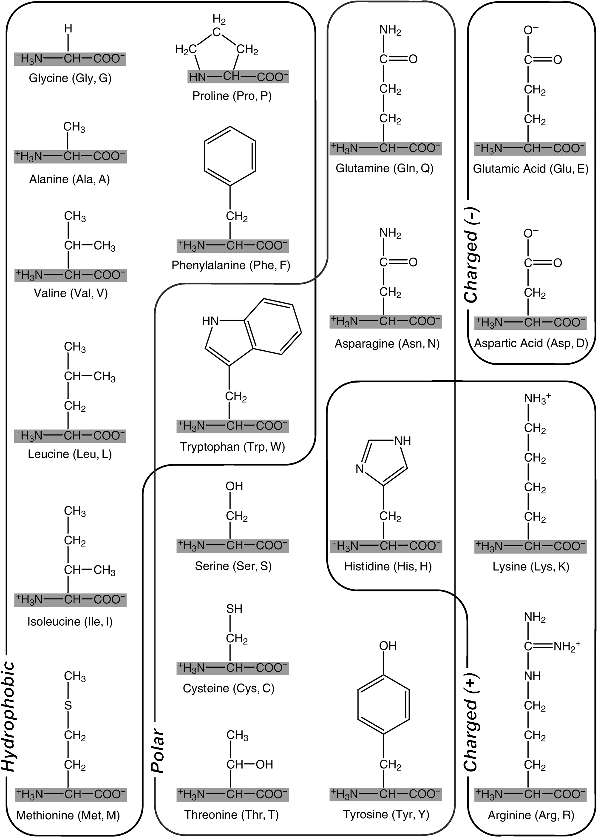
\includegraphics[width=0.8\textwidth]{wiley_liss_structural_bioinformatics_amino_acids.png}
	%\end{center}
	\caption{The 20 types of amino acid, each with a distinct side chain. In this figure, the carboxyl group has lost a hydrogen leaving a negative charge, and the amine group has gained a hydrogen leaving a positive charge. The elements which make up a peptide backbone are highlighted in gray, in addition to the hydrogen which connects to the $\alpha$-carbon. The side chains give rise to various electrical properties, as indicated by the circumscriptions. Taken from~\cite{scheeffink2003}.}
	\label{fig:aminoacids}
\end{figure}

Amino acids link together when the nitrogen atom from one protein's amine group bonds covalently with the carbon atom of another protein's carboxyl group, releasing a water molecule in the process.
This covalent bond is called a peptide bond, and an amino acid involved in at least one such bond is referred to as an \textit{amino acid residue}, or \textit{residue}.

A \textit{peptide}, or \textit{peptide chain}, is a linear chain of amino acids held together by peptide bonds, and the \textit{backbone} of the peptide consists of all atoms participating in peptide bonds together with the $\alpha$-carbons.
If a peptide contains several residues it is referred to as a \textit{polypeptide}.
Proteins consist of one or more polypeptides which are bound together.
All peptides have a natural ordering of their amino acid residues defined by the order in which they were incorporated into the peptide during protein synthesis.
The first residue to be incorporated has a free amine group denoted the \textit{N-terminus}, whereas the last residue has a free carboxyl group denoted the \textit{C-terminus}.


A residue's side chain can influence how it interacts with other amino acids or other atoms and molecules. For example, oppositely charged side chains will be attracted to each other, and polar and non-polar side chains will not strongly interact with each other. 
Polar side chains are also called hydrophilic due to their affinity for water, and non-polar side chains are also called hydrophobic for the opposite reason.
Residues in the same protein, by virtue of their spatial proximity, will tend to interact with one another. 
This influences the folding of the protein into a 3D structure.

%TODO: describe domains or motifs?
%TODO: mention globular proteins vs other kinds?


\subsection{Protein Structure}

Protein structure can be described via four levels of abstraction. 
\textit{Primary structure} refers to the sequence of amino acid residues (from N-terminus to C-terminus) in a single polypeptide, and is determined by the sequence of codons in the corresponding coding mRNA from which the protein is translated.
Sequences are typically written using a string of letters, where each unique letter corresponds to a different residue type. 

The physical chemistry associated with peptide bonds gives rise to the property that the Nitrogen and Carbon atoms involved in the peptide bond, along with the adjacent $\alpha$-carbons, all lie within a plane, denoted the \textit{amide plane}.
Each $\alpha$-carbon lies on the intersection between two amide planes, and the planes are free to rotate with respect to each other. 
Their relative orientation is described by two angles, $\psi$ and $\phi$, which describe the rotation of each plane with respect to the $\alpha$-carbon's tetrahedral geometry.
%TODO: figure?
In some cases, side chains prohibit certain angles due to \textit{steric constraints}, which enforce that no two atoms may occupy the same volume of space at the same time.
The angles $\phi$ and $\psi$ allow a certain amount of flexibility in the peptide backbone, which gives rise to higher order structures.

\textit{Secondary structure} describes the common local structures that arise from the interaction of non-adjacent residues in a polypeptide.
There are three such categories of local structures: helices, sheets, and loops.
A helix occurs when the polypeptide coils into a barrel-like structure (like the threads of a screw) and residues from adjacent coils form hydrogen bonds with one another.
There are multiple types of helices, as determined by the distance along the polypeptide backbone between two hydrogen bonded residues.
The most common type is the $\alpha$-helix, corresponding to a distance of three. 
%TODO: figure?
A sheet occurs when two non-adjacent sections of the polypeptide align next to each other such that residues in one of the sections form hydrogen bonds with residues in the other section.
Sheets may be parallel, in which the upstream portions (nearer the N-terminus) of each section bond with each other as well as the downstream portions (nearer the C-terminus), or anti-parallel, in which the upstream portion of one section bonds with the downstream portion of the other section, and vice versa.
%TODO: figure?
In either case, these are referred to as $\beta$-sheets. 
Some sections of the polypeptide may form neither helices nor sheets, and are sometimes called \textit{loops}.
These sections are more flexible than helices or sheets due the lack of hydrogen bonds, and therefore are useful in connecting the end of one helix/sheet to the beginning of another.

Helices and sheets provide some rigidity to a polypeptide, but it typically further "folds" together into a 3D structure.
This resulting 3D global structure is considered \textit{tertiary structure}.
Common collections of secondary structural elements are referred to as motifs and often have functional significance.
Larger subsections of a protein which maintain their general structure even if separated from the rest of the protein are called domains. 
Both motifs and domains play a significant role in protein function~\cite{scheeffink2003}.

Finally, in some cases multiple polypeptides combine together into a complex.
Because a polypeptide complex may perform a singular function that is not achievable by each of its constituent chains, it is sometimes considered a single protein.
In this case, the \textit{quaternary structure} describes the manner in which the individual polypeptides combine together to form the complex. 


\subsection{Protein Interfaces And Their Prediction}

%TODO: mention ligand and receptor

The locus of protein interaction is the interface, which is comprised of pairs of residues, one from each interacting protein, which interact with one another and bind the two proteins together.
Such interaction between residues requires electrochemical and geometric compatibility in the local neighborhood of a residue pair.
For example, like-charged residues will be counter-conducive to the formation of an interface due to mutual repulsion, and opposite-charged residues will have the opposite effect.
Polar residues are more likely to interact with other polar residues than with non-polar ones, and non-polar residues are more likely to interact with other non-polar residues than polar ones.
The notion of geometric compatibility suggests that portions of the interface on each protein should exhibit some form of shape complementarity with each other. 
Because these factors are relevant in the formation of interfaces, they are also important to the prediction of interfaces.

Historically, there have been two variants of the protein interface prediction problem: \textit{partner independent} and \textit{partner specific}.
The former variant considers a single residue from a protein and attempts to answer the question: does this residue form a part of the interface with a given partner protein?
The latter variant considers pairs of residues, each from a different protein, and attempts to answer a more specific question: does this \textit{pair} of residues constitute part of the interface between the two proteins?
The pairwise nature of partner specific prediction allows the consideration of the compatibility of a pair of residues, which has been found to increase performance~\cite{ahmad2011}.

Interfaces exhibit a local spatial correlation in that a residue is more likely to be a part of an interface if nearby residues are also a part of the interface. 
Local spatial correlation can aide prediction if information from nearby residues is taken into account during prediction.

In some cases, proteins undergo conformational change when binding because the presence of another protein changes the most energetically favorable state. 
In fact, sometimes this conformational change can actually facilitate the function of a protein or complex.
This can hinder prediction since the bound conformation is not known a priori and so the prediction must be made on the basis of the unbound protein structures. 

Methods of interface prediction include \textit{docking methods}, \textit{template-based methods}, and \textit{machine learning methods}.

Docking methods predict the 3D bound formation of two proteins in a complex and extract the interface from the predicted formation. 
These methods often use energy minimization techniques which account for shape complementarity~\cite{chen2003}\cite{zundert2016}.
Unlike template and machine learning methods, docking methods do not require a library of known interfaces in order to make predictions, but are historically poor at accounting for conformational change~\cite{ezkurdia2009}.

Template based methods make predictions based on similarity to a known template protein complex.
The protein of interest is compared to a library of proteins whose interface is known, and the interface for the protein of interest is predicted using the interfaces of similar proteins.
Template methods rely on a non-redundant template set of protein interfaces and compare entire interfaces to the templates~\cite{tuncbag2011}.

Machine learning methods attempt to directly predict the interface rather than comparing against a template complex or predicting the bound formation, however they still use information from a library of complexes whose interfaces are known.
Machine learning approaches have included use of a neural network~\cite{ahmad2011} and a support vector machine~\cite{minhas2014}.
The latest SVM based approach is called PArtner-specific Interacting Residue PREDictor (PAIRpred), and utilizes multiple radial basis function kernels.
PAIRpred incorporates both sequence and structural information of residues, and uses pairwise kernels which operate on pairs of residues.
The method performs well compared to existing docking and machine learning methods~\cite{minhas2014}.

%TODO: Talk about neural network approach


The work described in this paper performs partner specific interface prediction using a more sophisticated neural network architecture than previous methods. 


\section{Artificial Neural Networks}

\textit{Feed forward artificial neural networks}, or less formally, \textit{neural networks}, are a class of machine learning algorithm which are loosely inspired by neuroscientific models of how biological neural networks operate. 
In its most basic form, a (artificial) neural network is a parameterized function which accepts a vector of data as input and produces either a scalar or vector output.
For example, the input vector may be pixel values in an image of interest, and the output function may be a label applied to that image that indicates its content.
In this paper, the function is denoted $f(x|\Theta)$, where $x$ is the input vector and $\Theta$ is the complete set of parameters.
$f$ can be decomposed into a sequence of layers, $h_i(x_i|\Theta_i)$, which perform a comparatively simple mathematical operations on their input to produce an output.
By convention, the input vector is considered the first layer of a neural network even though it constitutes no operations. 
The output of the last layer is the output of the network. 
All intermediate layers are termed \textit{hidden layers}, each of which accepts the output of the preceding layer, performs a mathematical operation, and passes the output to the subsequent layer.
The number of layers in a neural network (besides the first layer) is its \textit{depth}, and the number of outputs of a given layer is denoted the number of \textit{units} (or \textit{neurons}) in that layer.
Figure \ref{fig:twolayernetwork} depicts a two layer neural network with three inputs, four units in the hidden layer, and two outputs. 

\begin{figure}
	\centering
	%\begin{center}
	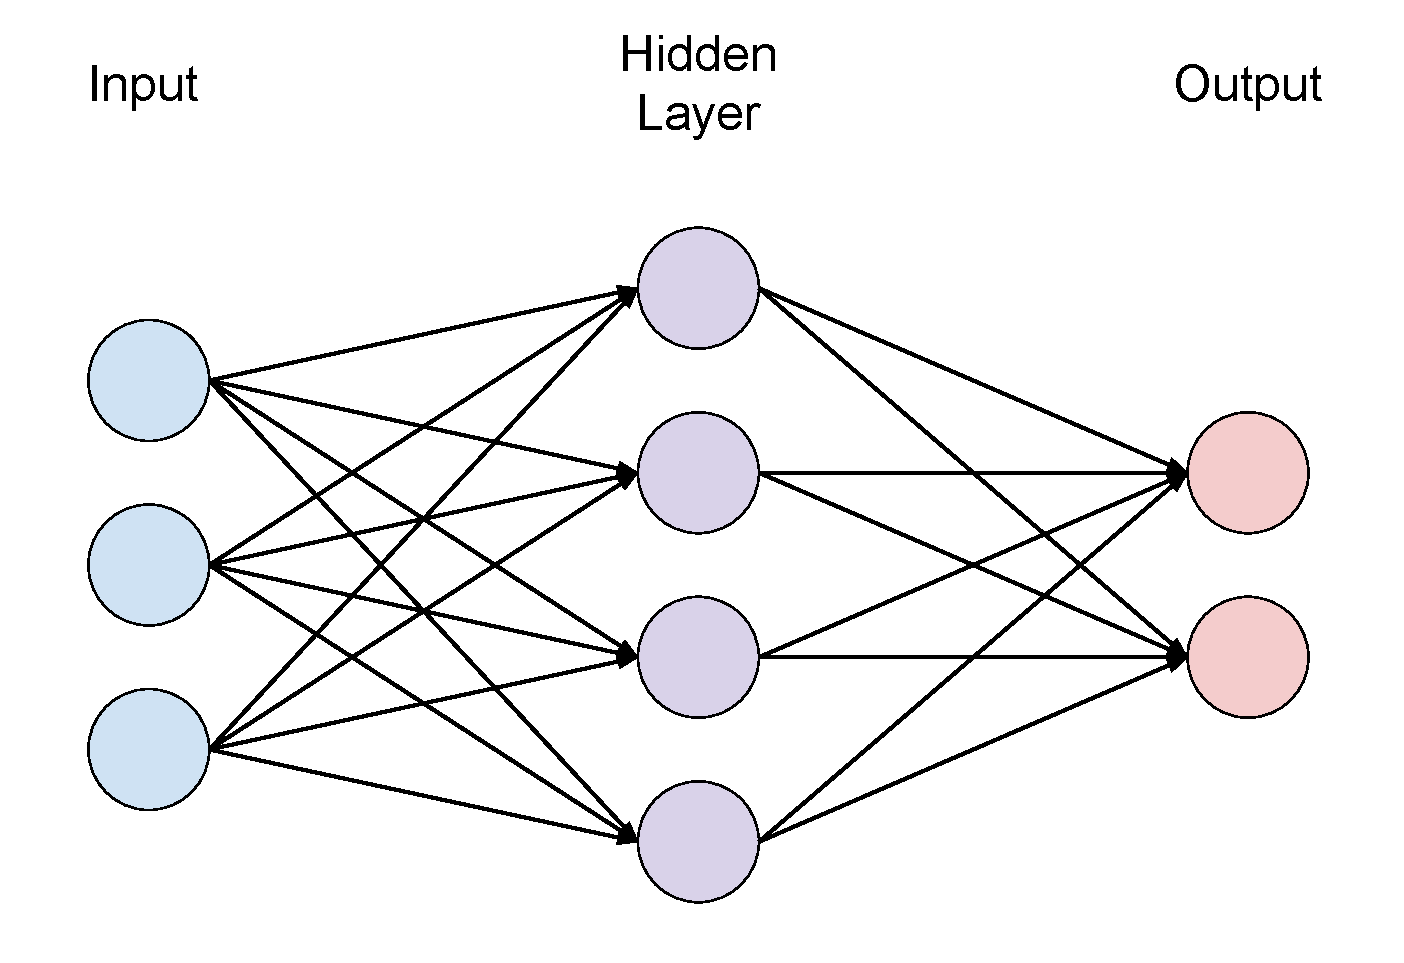
\includegraphics[width=0.8\textwidth]{twolayernetwork.pdf}
	%\end{center}
	\caption{A two layer neural network with a single hidden layer.}
	\label{fig:twolayernetwork}
\end{figure}

A common form of hidden layer is a \textit{dense layer}, in which each unit calculates a weighted sum of the layer inputs, where the set of weights is unique to each unit.
It is also common to add a scalar bias term and apply a sigmoid function on the weighted sum.
Dense layers have a convenient mathematical representation:

\begin{equation}
h(x|W, b)=\sigma(W x^T + b)
\label{eq:denselayer}
\end{equation}

\noindent
where $W$ is a matrix of weights, $x$ is the layer input, $b$ is a vector of biases, and $\sigma(\cdot)$ is a sigmoid function.
If there are $n$ inputs to a layer and $m$ units in the layer, then $W$ has shape $(n,m)$ and $b$ has shape $(1,m)$.
$W x^T + b$ is often called the \textit{signal}, and $h$ the \textit{activation}.

Despite being conceptually simple, this formulation of artificial neural networks is capable of approximating any continuous function on a compact subset in $\mathbb{R}$ with arbitrarily small error~\cite{cybenko1989}.
The challenge of using neural networks for function approximation is in finding the appropriate set of parameters to approximate the desired function.
For simple feed forward neural networks, this is accomplished by quantifying the error between the desired function and the approximation for given training data $X=(x_1, x_2, ..., x_N)$ with a differentiable loss function $L(\Theta | X)$. 
$f$ is updated by differentiating the loss function with respect to the network parameters $\Theta$ and "taking a step" in parameter space in the opposite direction of the gradient. 
This update step can be repeated iteratively in a process called \textit{gradient descent} and mathematically takes the form:
\begin{equation}
\Theta_{k+1} = \Theta_k - \eta \nabla L(\Theta_k | X) = \Theta_k - \eta \sum_{i=1}^{N} \nabla L(\Theta_k | x_n)
\label{eq:bgd}
\end{equation}

\noindent
where $\eta$ is a tunable step size and $k$ indicates the iteration.
Weights are usually initialized by drawing from distributions that have some empirical or theoretical justification~\cite{glorot2010}.
A variant of this algorithm, called \textit{stochastic gradient descent} performs an update using a gradient computed from a random subsample (without replacement) of the training data at each iteration.
When all training data has been sampled, this constitutes an \textit{epoch}.
%TODO: write about backpropagation? (and minibatching, etc...?)
Like many machine learning algorithms, neural networks risk \textit{overfitting}, in which the network learns to approximate the training data (which usually contain noise), rather than the underlying function from which the training data are assumed to be drawn.
This hinders the ability of neural networks to generalize to unseen data.

In recent years, more advanced forms of neural networks under the moniker \textit{deep learning} have demonstrated success in sophisticated tasks, particularly for those related to images~\cite{lecun2015}. 
These advances were catalyzed by the availability of large volumes of labeled image data and the improvements in computing power from general purpose graphical processing units (GP-GPUs) and distributed systems.
Such factors allow experimentation with larger networks and more complicated layer operations such as convolutions, which are described in the following section.

\subsection{Convolutional Neural Networks}

Traditionally, neural networks do not explicitly account for inherent structure in the input which may be useful when approximating the output function.
For example, pixels in an image are often spatially correlated, but spatial information is not explicitly given to the network when using dense layers.
Convolutional layers are one way to incorporate structure information in a neural network. 
The name comes from an interpretation of how they operate on a set of inputs with a well defined grid structure, such as a pixelated image or discrete time series, where a filter of weights (e.g. 3x3 pixels for images) is convolved over the input grid.
That is, at each filter position, the filter weights are multiplied with the corresponding inputs, called the \textit{receptive field}, and summed to produce a scalar value.
As with dense layers, the result is usually passed through a sigmoid function.
Because each filter multiplication is associated with a position of the input grid, the output retains a grid structure.
Figure \ref{fig:convolutionallayer} depicts a simple convolutional layer.
In color images, each pixel has multiple values, or \textit{channels}, which capture color information, and the filter must have the same number of channels as the input in order to take the elementwise product between the filter and the receptive field.
A convolutional layer may contain multiple filters, each of which produces a grid of scalar values which can be considered a channel in the output.
The weights in a filter determine which receptive fields produce a larger output and which do not, so a filter can be viewed as detecting specific patterns in a receptive field.
An alternate interpretation of convolutional layers is that weights are being shared across a layer such that each unit in the convolutional layer receives inputs from a different localized region of the input, and that all units share weights appropriately.

%TODO: equation?

\begin{figure}
	\centering
	%\begin{center}
	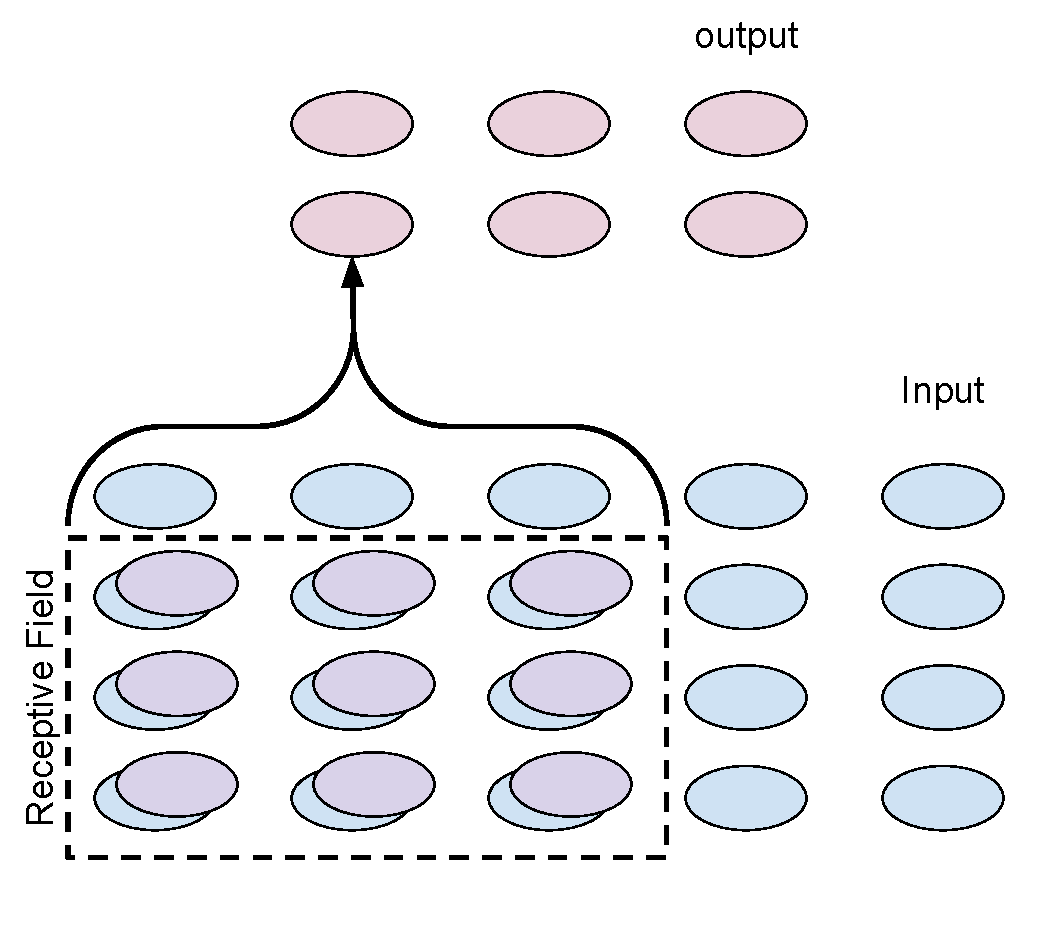
\includegraphics[width=0.8\textwidth]{convolutionallayer.pdf}
	%\end{center}
	\caption{A convolutional layer with a single 3x3 filter operating on a grid input with a single channel. The filter is multiplied elementwise with the corresponding inputs and produces a scalar value.}
	\label{fig:convolutionallayer}
\end{figure}


Convolutional layers exhibit certain properties which aid in image related tasks:
\begin{itemize}
\item
\textit{Local pattern detection}: Convolutional filters are usually significantly smaller than the size of the input, so for any given position of the filter they are operating on a local neighborhood of the input. 
This means that patterns detected by a particular filter are local.
\item
\textit{Global application}: Since filters are convolved over the input, patterns can be efficiently detected regardless of where they occur in the input.
In a dense layer, detection of a local pattern in each part of the input requires that weights associated with each region of the input be trained individually to detect the same pattern.
This means the training data must represent the same pattern in all portions of the input. 
For example, to train a dense layer to detect a cat's ear regardless of where it appears in an image, it must be trained using data which represent a cat's ear in every possible position of the image.
\item
\textit{Stackability}: The output of a convolutional layer retains the same grid structure as the input, so the output of a convolutional layer can be used as input to another convolutional layer.
Consider a neural network with two convolutional layers stacked on top of one another.
The receptive field of a unit in the second layer consists of units in the preceeding convolutional layer, each of which has its own receptive field in the input.
Hence filters in the second layer detect patterns of patterns in the original input, which suggests that stacked layers learn a hierarchical representation of the original input.
Furthermore, stacked layers have effectively larger receptive fields on the original input, and are therefore able to detect larger patterns in the original input.
The ability to learn a conceptual hierarchy of patterns in the input, from simple textures and edges to complex objects like faces or vehicles, has been demonstrated empirically as well~\cite{zeiler2013}.
\item
\textit{Robustness to overfitting}: The weight sharing inherent in convolutional layers means there are fewer trainable weights compared to a dense layer with the same number of hidden units. 
This reduces the propensity of the network to overfit to the training data and improves its ability to generalize to unseen examples.
\end{itemize}

Convolutional neural networks often incorporate \textit{pooling layers}, which reduce a small region of a grid (e.g. 2x2 pixels for an image) to a single grid element that takes either the maximum or average value (per channel) of the region. 
Pooling allows downsampling of the grid, and is often performed between convolutional layers. 

The convolutions described above can only operate on a regular grid. 
Proteins, however, have inherently irregular structure. 
In this work we adapt the notion of convolution to work with irregular structure, which are represented as graphs, which is described in Chapter \ref{chap:methods}.





